 \documentclass[12pt]{article}
\usepackage[english]{babel}
\usepackage[utf8x]{inputenc}
\usepackage{amsmath}
\usepackage{graphicx}
\usepackage{float}
\usepackage[colorinlistoftodos]{todonotes}

\begin{document}
\begin{titlepage}
\newcommand{\HRule}{\rule{\linewidth}{0.5mm}} 

\center 

\textsc{\LARGE Universistat Polit\`{e}cnica de Calatunya}\\[1.5cm]

\includegraphics[scale=0.2]{Upc.PNG} \\[1cm]
\textsc{\Large Statistical Modelling and Design of Experiments}\\[0.5cm] 
\textsc{\normalsize Master in Innovation and Research in Informatics}\\[0.5cm] 

\HRule \\[0.4cm]
{ \Large \bfseries Assignment 2}\\[0.4cm]
\HRule \\[1.5cm]

\begin{minipage}{0.4\textwidth}
\begin{flushleft} \large
\emph{Author:}\\
First name \textsc{Daniel Pujazon Bonet}\\
\end{flushleft}

\end{minipage}\\[2cm]

{\large \today}\\[2cm]
\vfill

\end{titlepage}

\section {Generate your data.}
\vspace{5mm}
\subsection {Define, for each factor (from 1 to 5) a distribution (the RVGs that you prefer, uniform, normal, exponential, etc.). For the factors 6 to 10 define a function that uses the previous variables, as an example F6=F1+2F3.}
\subsection {Define an answer variable that will be composed by a function that combines a subset of the previous factors plus a normal distribution you know (to add some random noise).}
The data stream is generated through the attached DataGen.cpp file and it's save it on a .csv file called DataSet.csv (also there's a .txt file).\\
Take note that factors indexing (nomenclature) will start from 0. So the first 5 factors, defined by probability distributions, are F0, F1, F2, F3 and F4. The rest F5, F6, F7, F8, F9 and F10 are the factors resulting on a linear combination of the first 5 factors being the F10 the ASNWER output variable.

\section {Obtain an expression to generate new data.}
\vspace{5mm}
\textbf{Imagine that you don’t know nothing regarding how this dataset has been generated. Consider that the factors represent different machines and the answer is the time to do an operation.\\
You need to explore it because you want to define a model to obtain new data for your DOE (you want to detect the possible relations and the interactions between the factors, or maybe you want to test alternatives or predict future scenarios).}
\subsection {Explore the possible relations of all the factors and the answer variable, you can use any technique developed during the course (LRM or ANOVA).}

We are gonna to do a PCA due to know the iterrelation between the different factors. After that we will generate some Linear Regresion models (LRM) and we will take the one that fits better our requirements. All will be made through the R script ObtainExpresion.r\\
So, applying PCA to the DataSet.csv we have found:\\

\begin{itemize}
\item After PCA (Figure 1) we see that F3, F8, F6, F1, F7 and F2 are strong correlated. F3,F8 and F6 are positive correlated while F1, F7 and F2 are negative correlated.\\ On the other side, F0, F5, F4 and F9 are strong and positive correlated.
\item Each group angle respect to one of the axis is near to 0, what means that these group is fully explained only by one PC: First group (F3,F8...) is almost parallel to y-axis, PC2, while second one (F0, F5...) is almost parallel to x-axis, PC1. 
This means that the other-PC group variables has no effect (because they're independant or because the impact of the other variable on the result it's too weak) on the value of the ohter-PC group vairables (pe: F5 value is not significantly determined by F3, F6 is not determined by F0... and so on)
\item Scree plot (placed below) show us that we need at least 4 variables to explain more than the 80\% of the system variables variation (even if we go further, with 5 variables we explain 100\% of variability so this means that from 6th variable, which explain 0\% of the variance, are full explained by the other variables).
\end{itemize}
\newpage
\begin{figure}[!htb]
    \centering
	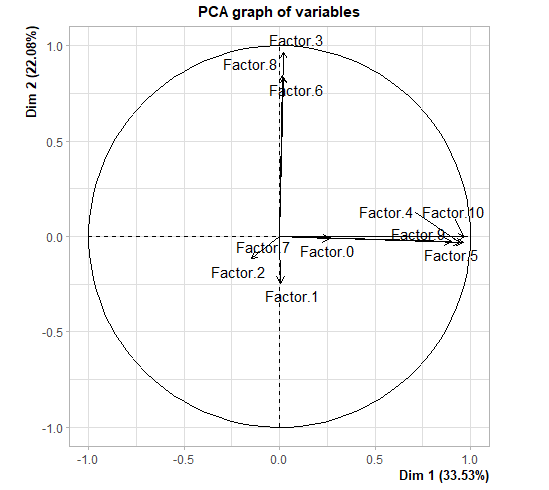
\includegraphics[scale=0.7]{pca.PNG}
    \caption{Spatial density of space debris ranging from 1cm to 10cm.}
    \label{top}
\end{figure} 
\begin{figure}[!htb]
    \centering
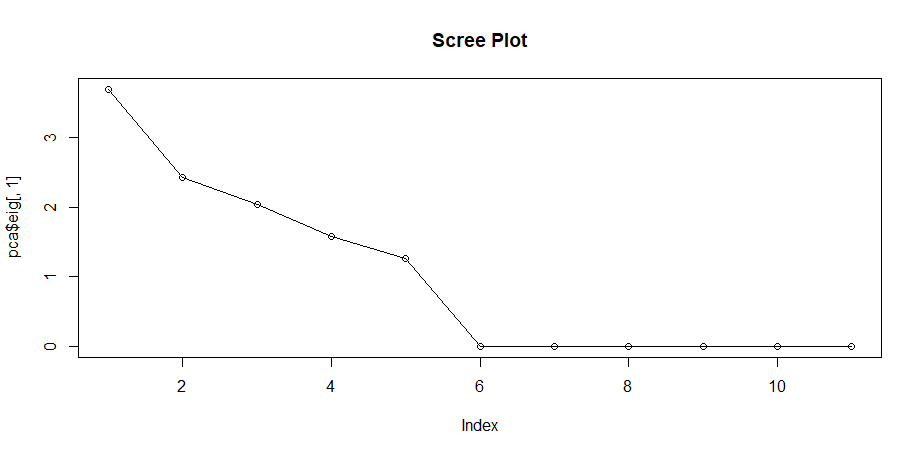
\includegraphics[scale=0.5]{screeploot.png}
    \caption{Spatial density of space debris larger than 10cm.} 
    \label{bottom}
\end{figure} 
\newpage
So, knowing that there are 5 variables that explain 100\%, we could do all the possible LRM using 5 of the 10 variables (which would be 252, combination without repetitions of 10 elements taken from 5 to 5) and we will get the one that fit better. \\

A LRM with all variables of course exlpain 100\% of the variation on answer.
A LRM2 with all the F1,F2,F3,F4,F5 (without F0) variables explain also the 100\%.
On LRM3 if we only take the first 4 factors (as scree plot conclusions). With that we only can explain the 78\%, so we will use the or LRM2 or LRM4. Take a look that p-value is higher than accepted value so we won't use it:\\
$(LRM2) Answer = +5(X1)-3(X2)-5(X3)-1.18*10^{-6}(X4)+(X5)$\\
$(LRM4) Answer = +4(X0)+5(X1)-3(X2)-5(X3)+(X4)$\\

If we compare both, all variables on both LRM have the same p-value (so more or we see that LRM2 X4 has bigger p-value than X3 on LRM3. Also residual standrad error on LRM4 is smaller than LRM2, so we would pick LRM2 instead of LRM4.\\
The last check between two models will be based on code them and operational validate with the system applying the inputs from DataSet and compare both outputs with the DataSet answer. This is made on DataGen.cpp and dumped on testLRM.txt. We can see how LRM4 outputs are more near to answer than LRM2. So let's use LRM4. \\
We also have tested the assumptions of linear regresion models (Can be seen on ObtainExpression.R)\\
\subsection {Describe what you find on this analysis and, explain if it is coherent with the knowledge you have from the data.}
\begin{itemize}
\item  First of all, the scree plot is coherent with the fact that from Factor6 to Factor10 are totally and only dependant on the first 5 factors.
\item Also is coherent that F8,F6 and F7 are strongly correlated with F3, F2 and F1. Their definitions are: F6=$F1 + 3*F3$; F7=$2*F2 + 3*F2$; F8=$F3 - F1$
\\The signs inside each function also explains why, for example, F8 is negative correlated with F1.
\item On the same way correlation between F5, F9 with F0 and F4 make sense:
F5=$4*F0 + F4$; F9=$F4 - F0$.
\item If we calculus theoretically the Answer function ,being decomposed on the independant factors, we obtan the same one as LRM4.

\end{itemize}
\newpage
\subsection {Use a simulation model to generate new data. The simulation model will be a very simple model composed by one server by each one of the factors you use on the answer.}
\noindent\begin{minipage}{0.3\textwidth}% adapt widths of minipages to your needs
  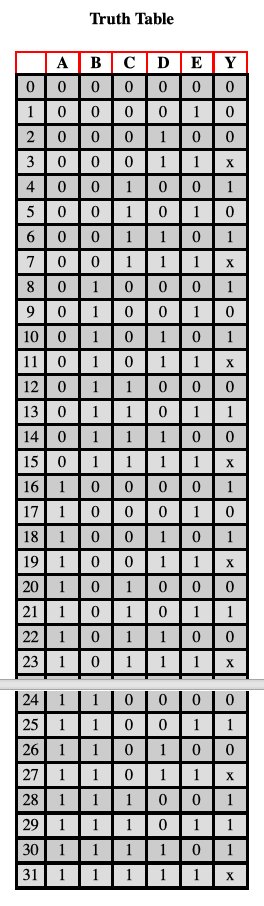
\includegraphics[scale=0.4]{scenariosFullFactor.png}
\end{minipage}%
\hfill%
\begin{minipage}{0.6\textwidth}\raggedright
We are going to implement the model defined previously with GPSS World. For doing that we will base on the 2k factorial design explained on the following section. It's the attached file M2.gps and has been deployed with GPSS World.\\
The idea is, you define which scenario are you going to simulate on the SCENARIO variable according to the truth table (pe: SCENARIO 3 means F0 (-), F1 (-), F2 (-), F3 (+), F4(+). Then there's a function for each Factor which has the value, already calculated, for both (+) and (-) scenarios. First attempt was using queues (interpreting factors values as time) but distributions give us negative times so it make no sense. Then it's assigned to a ANSWER variable and dumped.\\
The REPETITIONS variable allows you to execute given SCENARIO as much as its specified.\\
Also added Random delay using RN1 that adds random noise to whole REPETITIONS executions of SCENARIO. We don't update it with RMULT so each new simulation follows the same random distribution, but random at the end.
\end{minipage}

\newpage
\section {DOE}
\vspace{5mm}
\textbf{Now you have a model to generate new data. This model can be used to generate data for the different scenarios that must be considered.}
\subsection {Define a DOE to explore with what parametrization of the 10 factors the answer obtains the best value (define what means best, i.e. maximize or minimize the value).}
\subsection {Detect and analyze the interactions.}
Let's do step by step

\subsubsection{Experiment objectives.}
What we have are different kinds of machines used for execute the program (the different factors). Inside each kind of machines some of them can be faster and some of them slower (that are the different levels that we see on each factor). So having one machine of each type, when we run a program it executes on a T time.\\
The objective of the experiment is try to minimize the T time execution. This can be done if we know which kind of machine has the biggest effect on the execution time (also if there's relation between types of machines that are significant to the T execution time...).

\subsubsection{Experiment process variables.}
The dataset provided has different executions (rows) with 10 kinds of machines (factors), each one with a specific times (levels), and finally the T execution time (response variable). \\
We don't know if there are any other issue on each kind of machine or somewhere that is affecting the T execution time, so we assum that degree of randomness out of these variables.\\
With the system analysis done previosuly (the 1st point) we have seen that there are really only 5 kinds of machines that are significant on the T execution time. Then we are going to select that 5 different kinds of machines (A,B,C,D,E) as the process variable. Of course the T execution time is the response variable.


With all that system analysis we have been able to generate a model and we have been validated it after coding with GPSS (and in C) using the different values from dataset and comaprining them with the DataSet answers.

\subsubsection{Experimental design}
Firstly we want to see the global overview picture about the effect of each kind of machine and also the interactions between them. We can use a full factorial design. But seeing the dataset we realize that there are a lot of levels for each factor so it's not feasible. Then we deploy a 2k factorial design.\\

So, we have to define the maximum and minimum values for each factor. We will take the maximum and minimim values, (F5 has significant outliers so we take the minimum and maximum value at least with a 1\% of frequency to appear), from the empricial results (even we could also taken knowing the potential values that each distribution can generate. This is on ObtainExpresion.R):\\
\begin{itemize}
\item For Factor 1: (+):= 89.73; (-):= 12.50.
\item For Factor 2: (+):= 00.95; (-):= 6.25e-07.
\item For Factor 3: (+):= 49.97; (-):= 20.02.
\item For Factor 4: (+):= 02.16; (-):= 1.37.
\item For Factor 5: (+):= 31.1965; (-):= -20.162.
\end{itemize}
This means that, at least with our current design, we have 32 scenarios (on the truth table the '0' means the minimum value, (-), while the one is the maximum, (+) and A,B,C,D,E are the F0, F1, F2, F3, F4 factors respectively).\\

\subsubsection{Result interpretation: Effects, interactions...}
So we are going to execute on 2 steps our 2k factorial design: First of all we are going to execute all scenarios 10 times (pilot test) which will give us some results with a fiven confidence interval. With that we can calculus the required extra executions of each scenario with the desired accureacy and execute them.\\
The results of the 320 executions (10 times each scenario) are on Simulation1.csv.
Then, we calculate the confidence interval of each one using ModelPostProcessing.R. Can be seen on IC1.txt\\
With that 10 replications we already have a confidence interval smaller than 5\% (not for a few of them).\\

Now due to see the effect of each machine type and also the interactions between them, we can apply Yates algorithm (calculated with Yates.csv and also bigger):
(A is F0, B is F1...)
We can see how machines of type F1 have the biggest impact on adding time while the machines of type F3 are the ones that improves at most the speed (as bigger the level on that factor is bigger the negative part will be).\\
About interactions, we see that all have the same absolute value. This means that interactions between machines types has no significant effect on the T exe.\\
\textbf{So we can conclude that if we have to priorize one type machine for decreasing the Texe when a program is executed on a enviroment where at least 1 machine of each type is needed, you have to minimize the value of the F3 type machines}

\begin{table}[]
\scalebox{0.77}{
\begin{tabular}{llllllllllllll}
A & B & C & D & E & T exe  & (1)		& (2)		&(3)		&(4)		&(5)		&Div 	&Effect 		&Id\\
- & - & - & - & - & -28.7  &  -4,6 	 	&-7,7		&-373,1		&-397,9		&3840,7		&32		&120,021875		&Mean	\\		
- & - & - & - & + & 24.1   &  -3,1   	&-365,4		&-24,8		&4238,6		&1133,7		&16		&70,85625		&F5		\\	
- & - & - & + & - & -27.2  &  -182,6   	&12,8		&2101		&721,1		&310,3		&16		&19,39375		&F4		\\	
- & - & - & + & + & 24.1   &  -182,8   	&-37,6		&2137,6		&412,6		&307,7		&16		&19,23125		&F4F5	\\			
- & - & + & - & - & -116.9 &  6,4   	&1231		&206,7		&310,3		&-1128,3	&16		&-70,51875		&F3		\\	
- & - & + & - & + & -65.7  &  6,4   	&870		&514,4		&0			&305,9		&16		&19,11875		&F3F5	\\		
- & - & + & + & - & -117.1 &  -173,3   	&1248,4		&207		&307,7		&307,3		&16		&19,20625		&F3F4	\\		
- & - & + & + & + & -65.7  &  135,7   	&889,2		&205,6		&0			&310,7		&16		&19,41875		&F3F4F5	\\		
- & + & - & - & - & -22.5  &  615,5   	&104,1		&1,3		&-408,1		&384,9		&16		&24,05625		&F2		\\	
- & + & - & - & + & 28.9   &  615,5   	&102,6		&309		&-720,2		&306,3		&16		&19,14375		&F2F5	\\		
- & + & - & + & - & -22.5  &  435   	&102,8		&0			&307,3		&307,7		&16		&19,23125		&F2F4	\\		
- & + & - & + & + & 28.9   &  435   	&411,6		&0			&-1,4		&310,3		&16		&19,39375		&F2F4F5	\\		
- & + & + & - & - & -112.3 &  624,2   	&104,2		&-1,3		&307,3		&309,1		&16		&19,31875		&F2F3	\\		
- & + & + & - & + & -61.0  &  624,2   	&102,8		&309		&0			&311,7		&16		&19,48125		&F2F3F5	\\		
- & + & + & + & - & -112.3 &  444,6   	&102,8		&0			&310,7		&310,7		&16		&19,41875		&F2F3F4	\\		
- & + & + & + & + & 248.0  &  444,6   	&102,8		&0			&0			&307,3		&16		&19,20625		&F2F3F4F3\\			
+ & - & - & - & - & 281.7  &  52,8   	&1,5		&-357,7		&348,3		&4636,5		&16		&289,78125		&F1			\\
+ & - & - & - & + & 333.8  &  51,3   	&-0,2		&-50,4		&36,6		&-308,5		&16		&-19,28125		&F1F5		\\	
+ & - & - & + & - & 281.7  &  51,2   	&0			&-361		&307,7		&-310,3		&16		&-19,39375		&F1F4		\\	
+ & - & - & + & + & 333.8  &  51,4   	&309		&-359,2		&-1,4		&-307,7		&16		&-19,23125		&F1F4F5		\\	
+ & - & + & - & - & 191.8  &  51,4   	&0			&-1,5		&307,7		&-312,1		&16		&-19,50625		&F1F3		\\	
+ & - & + & - & + & 243.2  &  51,4   	&0			&308,8		&0			&-308,7		&16		&-19,29375		&F1F3F5		\\	
+ & - & + & + & - & 191.8  &  51,3   	&0			&-1,4		&310,3		&-307,3		&16		&-19,20625		&F1F3F4		\\	
+ & - & + & + & + & 243.2  &  360,3   	&0			&0			&0			&-310,7		&16		&-19,41875		&F1F3F4F5	\\		
+ & + & - & - & - & 286.4  &  52,1   	&-1,5		&-1,7		&307,3		&-311,7		&16		&-19,48125		&F1F2		\\	
+ & + & - & - & + & 337.8  &  52,1   	&0,2		&309		&1,8		&-309,1		&16		&-19,31875		&F1F2F5		\\	
+ & + & - & + & - & 286.4  &  51,4   	&0			&0			&310,3		&-307,7		&16		&-19,23125		&F1F2F4		\\	
+ & + & - & + & + & 337.8  &  51,4   	&309		&0			&1,4		&-310,3		&16		&-19,39375		&F1F2F4F5	\\		
+ & + & + & - & - & 196.6  &  51,4   	&0			&1,7		&310,7		&-305,5		&16		&-19,09375		&F1F2F3		\\	
+ & + & + & - & + & 248.0  &  51,4   	&0			&309		&0			&-308,9		&16		&-19,30625		&F1F2F3F5	\\		
+ & + & + & + & - & 196.6  &  51,4   	&0			&0			&307,3		&-310,7		&16		&-19,41875		&F1F2F3F4	\\		
+ & + & + & + & + & 248.0  &  51,4   	&0			&0			&0			&-307,3		&16		&-19,20625		&F1F2F3F4F3			
\end{tabular}
}
\end{table}

\end{document}